%%==================================================================%%
%% Author : Tejedo Gonz�lez, Daniel                                 %%
%%          S�nchez Barreiro, Pablo                                 %%
%% Version: 1.0, 28/11/2012                                         %%                   %%                                                                  %%
%% Memoria del Proyecto Fin de Carrera                              %%
%% Validation Framework, archivo ra�z                                       %%
%%==================================================================%%

\chapterheader{Validaci�n de las sintaxis concretas}{Validaci�n de las sintaxis concretas}
\label{chap:emfvf}

Este cap�tulo trata de describir el desarrollo de la tarea de implementaci�n del proceso de validaci�n de las sintaxis concretas. La validaci�n consiste en tratar de averiguar si ciertos aspectos de la sintaxis concreta construida que no se pueden comprobar mediante la gram�tica y el metamodelo son correctos. Un ejemplo de uno de esos aspectos es si la direcci�n introducida en el import para el modelo de caracter�sticas es correcta.

\chaptertoc

\section{Captura de requisitos}
\label{sec:emfvf:req}
%%==================================================================%%
%% Author : Tejedo Gonz�lez, Daniel                                 %%
%%          S�nchez Barreiro, Pablo                                 %%
%% Version: 1.0, 25/11/2012                                         %%
%% Version: 2.0, 06/02/2013                                         %%
%%                                                                  %%
%% Memoria del Proyecto Fin de Carrera                              %%
%% Sintaxis abstracta, requisitos                                   %%
%%==================================================================%%

El primer paso para desarrollar nuestro lenguaje era conocer qu� aspecto deb�a tener nuestro lenguaje y qu� restricciones deb�a satisfacer. Es decir, en primer lugar debemos realizar un proceso que podemos denominar de captura de requisitos para poder comprender qu� es lo que tiene que hacer exactamente el lenguaje que se pretende crear.

Concretamente nuestro lenguaje hab�a sido pr�cticamente definido por el profesor Pablo S�nchez, del Departamento de Matem�ticas, Estad�stica y Computaci�n de la Universidad de Cantabria, mediante notaci�n BNF. Dicha gram�tica, se muestra en la Figura~\ref{fig:constraintBNF}. Las ideas subyacentes a dicho lenguaje son las que se describen a continuaci�n. 

\begin{figure}[!tb]
    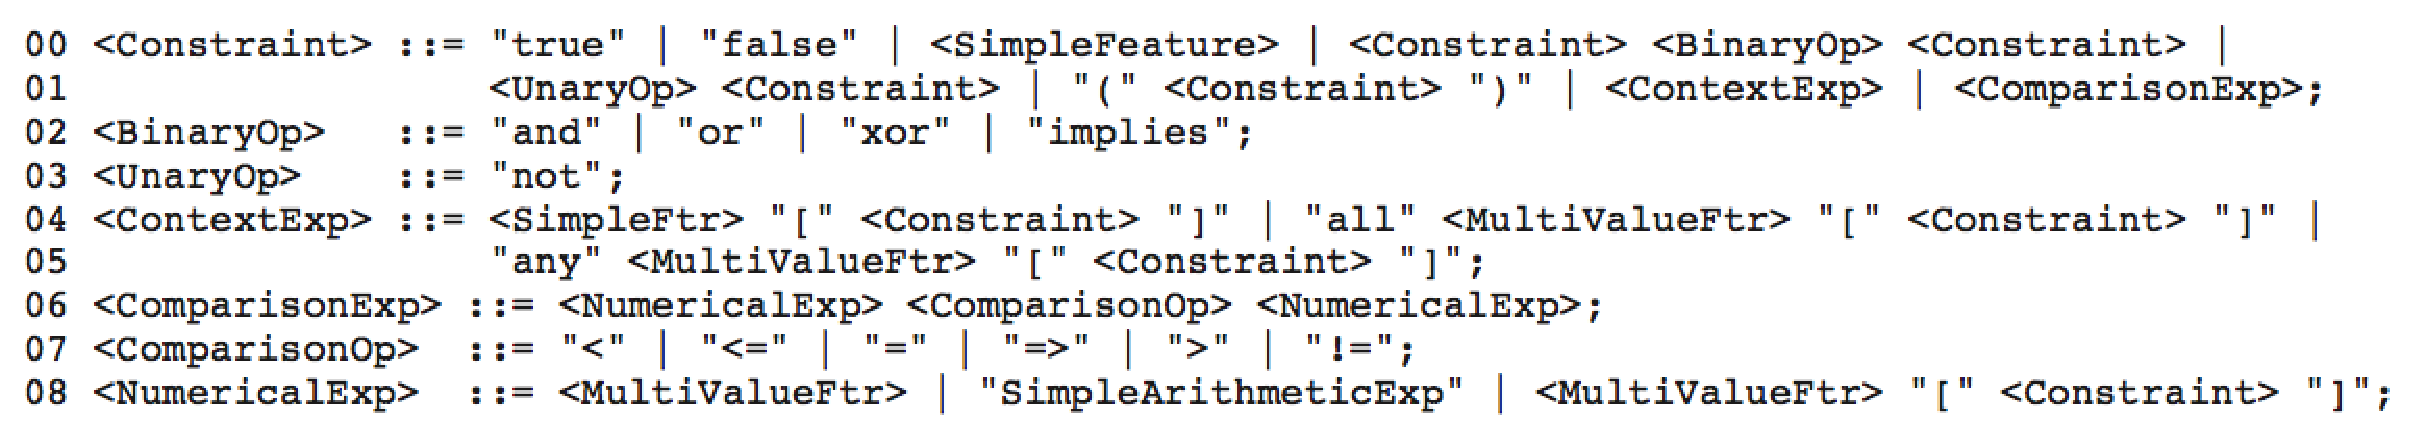
\includegraphics[scale=0.3]{metamodelo/constraintBNF.eps}
    \caption{Gram�tica en notaci�n BNF del lenguaje HCL}
    \label{fig:constraintBNF}
\end{figure}

En dicho lenguaje, una \emph{restricci�n} es una expresi�n l�gica que se puede evaluar a verdadero o falso. Una restricci�n puede ser simplemente un literal, es decir, $true$ o $false$, que se evaluar� a verdadero y falso respectivamente. Una restricci�n tambi�n puede ser una caracter�stica simple, es decir, una caracter�stica que puede aparecer en las configuraciones como m�ximo una vez. Una caracter�stica simple se eval�a a verdadero si ha sido seleccionada, y a falso en caso contrario.

Las caracter�sticas clonables son aquellas que pueden ser seleccionadas m�s de una vez en las configuraciones que construyamos sobre nuestro �rbol de caracter�sticas. Una caracter�stica clonable se eval�an como un n�mero entero positivo, incluido el cero. Ese n�mero representa el n�mero de clones que la caracter�stica posee dentro de una configuraci�n, o dicho de otro modo, el n�mero de veces que ha sido seleccionada. El hecho de que se eval�en como si fueran n�meros permite la inclusi�n de operaciones de comparaci�n entre distintas caracter�sticas clonables. Las operaciones de comparaci�n que se han de implementar son las siguientes: $<$,$<$=,$>$,$>=$,$=$,$!=$. Adem�s, tambi�n se puede utilizar el valor de las caracter�sticas clonables para implementar operaciones aritm�ticas b�sicas, tales como la suma, la resta, la multiplicaci�n y la divisi�n. Estas expresiones a su vez se pueden utilizar como subexpresiones, u operandos, dentro de las operaciones de comparaci�n. Las expresiones de comparaci�n se eval�an a verdadero o falso, y tambi�n pueden ser usadas como subexpresiones para crear expresiones l�gicas m�s complejas.

%%============================================================================%%
%% NOTA(Pablo) : Poner un ejemplo de este tipo de restricciones y explicarlas %%
%%============================================================================%%

Tal y como muestra la Figura~\ref{fig:constraintBNF}, una restricci�n tambi�n puede especificar un contexto concreto en el que poder evaluarla. Esto puede hacerse de varias maneras. Se puede especificar un contexto para una restricci�n poni�ndola entre corchetes y especificando el nombre de una caracter�stica al principio de la expresi�n. La caracter�stica usada como contexto puede ser tanto simple como m�ltiple. En el primer caso, la restricci�n s�lo ser� evaluada en el sub�rbol de la configuraci�n cuya ra�z sea la caracter�stica especificada.

%%============================================================================%%
%% NOTA(Pablo) : Poner un ejemplo y explicarlo                                %%
%%============================================================================%%

En el segundo caso entran en juego los operadores $all$ (para todo) y $any$ (existe). La operaci�n $all$ solo se evaluar� a verdadero si la restricci�n entre corchetes se cumple para todas las instancias de la caracter�stica clonable que act�a como contexto. En caso contrario, la operaci�n se evaluar� a falso. La operaci�n $any$ se evaluar� a verdadero si la restricci�n entre corchetes se cumple al menos una vez para todas las instancia de la caracter�stica clonable que act�a como contexto. Si la restricci�n no se cumple para ninguna de las selecciones, la operaci�n $any$ se evaluar� a falso.

%%============================================================================%%
%% NOTA(Pablo) : Poner un ejemplo y explicarlo                                %%
%%============================================================================%%

Merece la pena se�alar que una caracter�stica puede ser considera simple en un contexto determinado y clonable o m�ltiple en otro. Por ejemplo, la caracter�stica $LightMng$ es clonable en el contexto de $RoomFacilities$, pero simple en el contexto de $GeneralFacilities$. Debido a eso la caracter�stica $LightMng$ no puede ser utilizada sin especificar el contexto en el que est� ubicada, pues podr�a provocar un resultado no esperado o err�neo.

En la restricci�n $any Room[RoomFacilities[LightMng]]$ se pueden apreciar los dos diferentes usos para la operaci�n de contexto. Los corchetes externos indican a la operaci�n any que hay que aplicar la restricci�n a todas las habitaciones. Los corchetes internos indican que la caracter�stica $LightMng$ a la que se est� haciendo referencia es la hija de $RoomFacilities$ y no cualquier otra.

Adem�s nuestro lenguaje deb�a permitir vincular un modelo de caracter�sticas sobre el cual se definir�n un conjunto de restricciones externas. Este modelo se utilizar�, por ejemplo, para comprobar que los s�mbolos que aparecen como nombres de caracter�sticas en las restricciones se refieren a caracter�sticas que realmente existen en el �rbol de caracter�sticas. Por ejemplo, una restricci�n del tipo $AdvancedHeating => Heating$ carecer�a de sentido si algunas de las caracter�sticas $AdvancedHeating$ o $Heating$ no apareciesen en el �rbol de caracter�sticas sobre el cual estamos definiendo restricciones.

%%======================================================================================%%
%% NOTA(Pablo): Esto posiblemente sobre al introducir la traducci�n de la Secci�n III.
%%              Si es as�, eliminarla.
%%              Si los conceptos de restricci�n con contexto y operaci�n cuantificada
%%              no apareciesen, meter esta clasificaci�n pero resumida
%%======================================================================================%%
%%
%% De entre todos esos requisitos b�sicos, es necesario entrar en detalle en el n�mero 3
%% y enumerar la lista de operaciones que pueden ser definidas por nuestro lenguaje. Se
%% pueden clasificar en los siguientes tipos: \\
%%
%% - L�gicas: Son operaciones cuyos operandos han de ser caracter�sticas sin
%%   cardinalidad (tambi�n llamadas caracter�sticas simples), y que se evaluan a
%%   verdadero o falso. Entre las operaciones l�gicas encontramos las cl�sicas not,
%%   and, or, xor e implica.
%%
%% - Num�ricas: Sus operandos han de ser caracter�sticas con cardinalidad (tambi�n
%%   llamadas caracter�sticas m�ltiples) o simplemente n�meros. Su resultado se evalua
%%   con un valor num�rico. Las operaciones num�ricas a implementar son la suma, resta,
%%   multiplicaci�n y divisi�n.
%%
%% - Comparativas: Sus operandos han de ser caracter�sticas m�ltiples o simplemente n�meros,
%%   pero su resultado se evalua con un valor booleano. Las operaciones de comparaci�n a
%%   implementar son igual que, mayor que, menor que, distinto que, mayor o igual que y menor
%%   o igual que.
%%
%% - Operaci�n de contexto: Operaci�n que permite hacer referencia a una caracter�stica
%%   hija de otra caracter�stica. Esta operaci�n tiene sentido para seleccionar
%%   caracter�sticas cuyo nombre pueda estar repetido pero que tengan contextos diferentes.
%%   Por ejemplo, en el modelo de caracter�sticas SmartHome de la figura \ref{figsmarthome}
%%   podemos observar que la caracter�stica HeaterMng est� presente en muchos contextos
%%   diferentes. Esta operaci�n es necesaria para poder saber con seguridad a cual de esos
%%   contextos estamos aplicando la restricci�n.
%%
%% - Operaci�n de selecci�n: Operaci�n que corresponde a los operadores l�gicos cl�sicos
%%   "para todo" o "existe", y que tiene la misma funcionalidad. Evalua si una restricci�n
%%   se cumple para todos los casos en que puede existir  o si se cumple en alguno de los
%%   casos. Por ejemplo, en el modelo de la figura \ref{figsmarthome} se podr�a evaluar una
%%   restricci�n para cada una de las habitaciones que hayan sido definidas, y saber si se
%%  cumple en todas, en alguna o en ninguna.
%%
%%======================================================================================%%

Utilizando esta informaci�n como base, procedimos a crear el correspondiente metamodelo en Ecore para nuestro lenguaje.




\section{Implementaci�n de la validaci�n}
\label{sec:emfvf:req}
%%==================================================================%%
%% Author : Tejedo Gonz�lez, Daniel                                 %%
%%          S�nchez Barreiro, Pablo                                 %%
%% Version: 1.0, 28/11/2012                                         %%
%% Version: 2.0, 06/02/2013                                         %%
%%                                                                  %%
%% Memoria del Proyecto Fin de Carrera                              %%
%% Validation Framework, implementacion                             %%
%%==================================================================%%

La sintaxis propia de Ecore no nos permite especificar ciertas restricciones que debe satisfacer nuestro metamodelo. Dichas restricciones, las cuales se enumeran a continuaci�n, deben comprobar que:

\begin{enumerate}
    \item La ruta que indica donde est� el �rbol de caracter�sticas al que se
        aplican las restricciones definidas es correctas. Ello implica comprobar tanto que la ruta es correcta como que el fichero que se halla en dicha ruta corresponde de verdad a un �rbol de caracter�sticas.
    \item El atributo \emph{featureName} asociado a una \emph{SimpleFeature} o a una \emph{MultipleFeature} corresponde al nombre de una caracter�stica perteneciente al �rbol de caracter�sticas referenciado.
    \item Una caracter�stica identificada como \emph{SimpleFeature} en el modelo de restricciones (eval�a a verdadero o falso) es realmente una caracter�stica simple (no clonable) en el �rbol de caracter�sticas asociado. Sin esta comprobaci�n, podr�amos, por ejemplo, introducir caracter�sticas m�ltiples como operandos de operadores booleanas como \emph{and} u \emph{or}. En ese caso, ser�a imposible evaluar dichas operaciones ya que no podemos evaluar sus operandos a verdadero o falso.
\end{enumerate}

Respecto a la segunda restricci�n, merece la pena aclarar que el caso contrario, comprobar que una caracter�sticas considerada como m�ltiple en una restricci�n realmente lo sea, no es necesario controlarlo. La raz�n es que las caracter�sticas simples pueden tratarse como un caso particular o subtipo de caracter�stica m�ltiples, ya que siempre podremos considerarla como una caracter�stica clonable con cardinalidad $<0,1>$.

Para implementar estas restricciones externas se ha utilizado \emph{EMF Validation Framework}, herramienta integrada en EMF para este prop�sito concreto. Siguiendo las instrucciones proporcionadas por esta herramienta, a�adimos un m�todo de validaci�n a cada metaclase que necesitaba ser validada. En nuestro caso, dichas clases eran \emph{Model}, \emph{SimpleFeature} y \emph{MultipleFeature}. De acuerdo con las normas establecida por \emph{EMF Validation Framework}, dichos m�todos deben poseer un perfil concreto. Dicho perfil est� compuesto por dos par�metros, uno llamado \emph{diagnostics} del tipo \emph{EDiagnosticChain} y otro llamado \emph{context} que es un mapa \todo{cual es la clave y cual es valor de este mapa?}. Los m�todos de validaci�n han de retornar siempre un valor booleano.

Si la validaci�n es satisfactoria, el m�todo debe obviamente devolver un valor verdadero. En caso contrario, retornar� falso. El par�metro \emph{diagnostics} es un par�metro de salida que almacena informaci�n sobre el resultado de la validaci�n, tal como el tipo de error producido o el mensaje de error que queremos mostrar al usuario.

%%==========================================================================================%%
%% NOTA(Pablo): Explicar para qu� sirve el mapa                                             %%
%%==========================================================================================%%

Para implementar la primera restricci�n de las comentadas anteriormente, validar que la ruta que indica el �rbol de caracter�sticas sea v�lida y apunte realmente a un �rbol de caracter�sticas, se a�adi� un m�todo de validaci�n a la clase \emph{Model}. Para llevar a cabo esta validaci�n simplemente se carga el fichero existente en la direcci�n indicada y se controla las posibles excepciones que una direcci�n err�nea pueda generar. Adem�s, se comprueba que el contenido de esa direcci�n sea un �rbol de caracter�sticas. Se aprovecha tambi�n para generar una variable global que contenga el modelo le�do, ya que ser� necesario volver a cargarlo en posteriores comprobaciones.

Para implementar la segunda restricci�n, comprobar que la existencia de las caracter�sticas escritas en nuestro fichero de restricciones en el �rbol de caracter�sticas anteriormente asociado, a�adimos m�todos de validaci�n a las metaclases \emph{MultipleFeature} y \emph{SimpleFeature}. Para ello simplemente buscamos que el nombre almacenado en el par�metro \emph{featureName} de dichas metaclases corresponda con el nombre de alguna caracter�sticas del modelo cargado anteriormente. 

Para implementar la segunda restricci�n, que las caracter�sticas identificadas como simples realmente sean realmente simples en el �rbol de caracter�sticas asociado, a�adimos un m�todo de validaci�n a la clase \emph{SimpleFeature}. Para realizar la comprobaci�n tenemos que corroborar que �sta no pueda ser instanciada en m�s de una ocasi�n. Para ello tenemos que calcular la cota superior de su cardinalidad. Si dicha cota fuese mayor que uno, no ser�a una caracter�sticas simple. Este l�mite puede ser superior a uno en el caso de las caracter�sticas clonables, o de la caracter�sticas hijas de caracter�sticas m�ltiples. 

Tras a�adir estas restricciones estaba definida la sintaxis abstracta para nuestro lenguaje. Antes de proceder a la definici�n de una sintaxis concreta para dicho lenguaje, realizamos una serie de pruebas destinadas a verificar que el metamodelo creado recoge la sintaxis abstracta deseada. 
